\chapter{Concept Development}
\label{conception}

After the \textit{Museum für Ur- und Frühgeschichte Thürigens} was chosen as a partner, all previous ideas had to be analyzed more thoroughly with feasibility in mind. Thus, impractical, and too complex or too simple ideas were eliminated in two rounds of review. At first, vague ideas were either improved or discarded. Hence, a screen displaying only information about a fossilized fireplace was eliminated. The idea of a system for digitizing stone carvings was considered too complex to realize and therefore discarded as well. Afterwards, some of the museum's staff and I looked at the contents, that could be provided for the remaining candidates. This left us with two remaining possibilities, that were promising enough from an educational as well as a technical standpoint. The first one was the reproduction of the \textit{Fürstengrab von Haßleben}, which contains replicas and original artifacts from a 1700 year old grave of a Teutonic princess. A close second was a workshop, which should have shown how archeologists and restorers work behind the scenes of a museum. Here, the latter consisted of too many single parts and a lot of questions remained unanswered.

%\begin{figure}[H] % [H] -> Here!
	%\centering
	%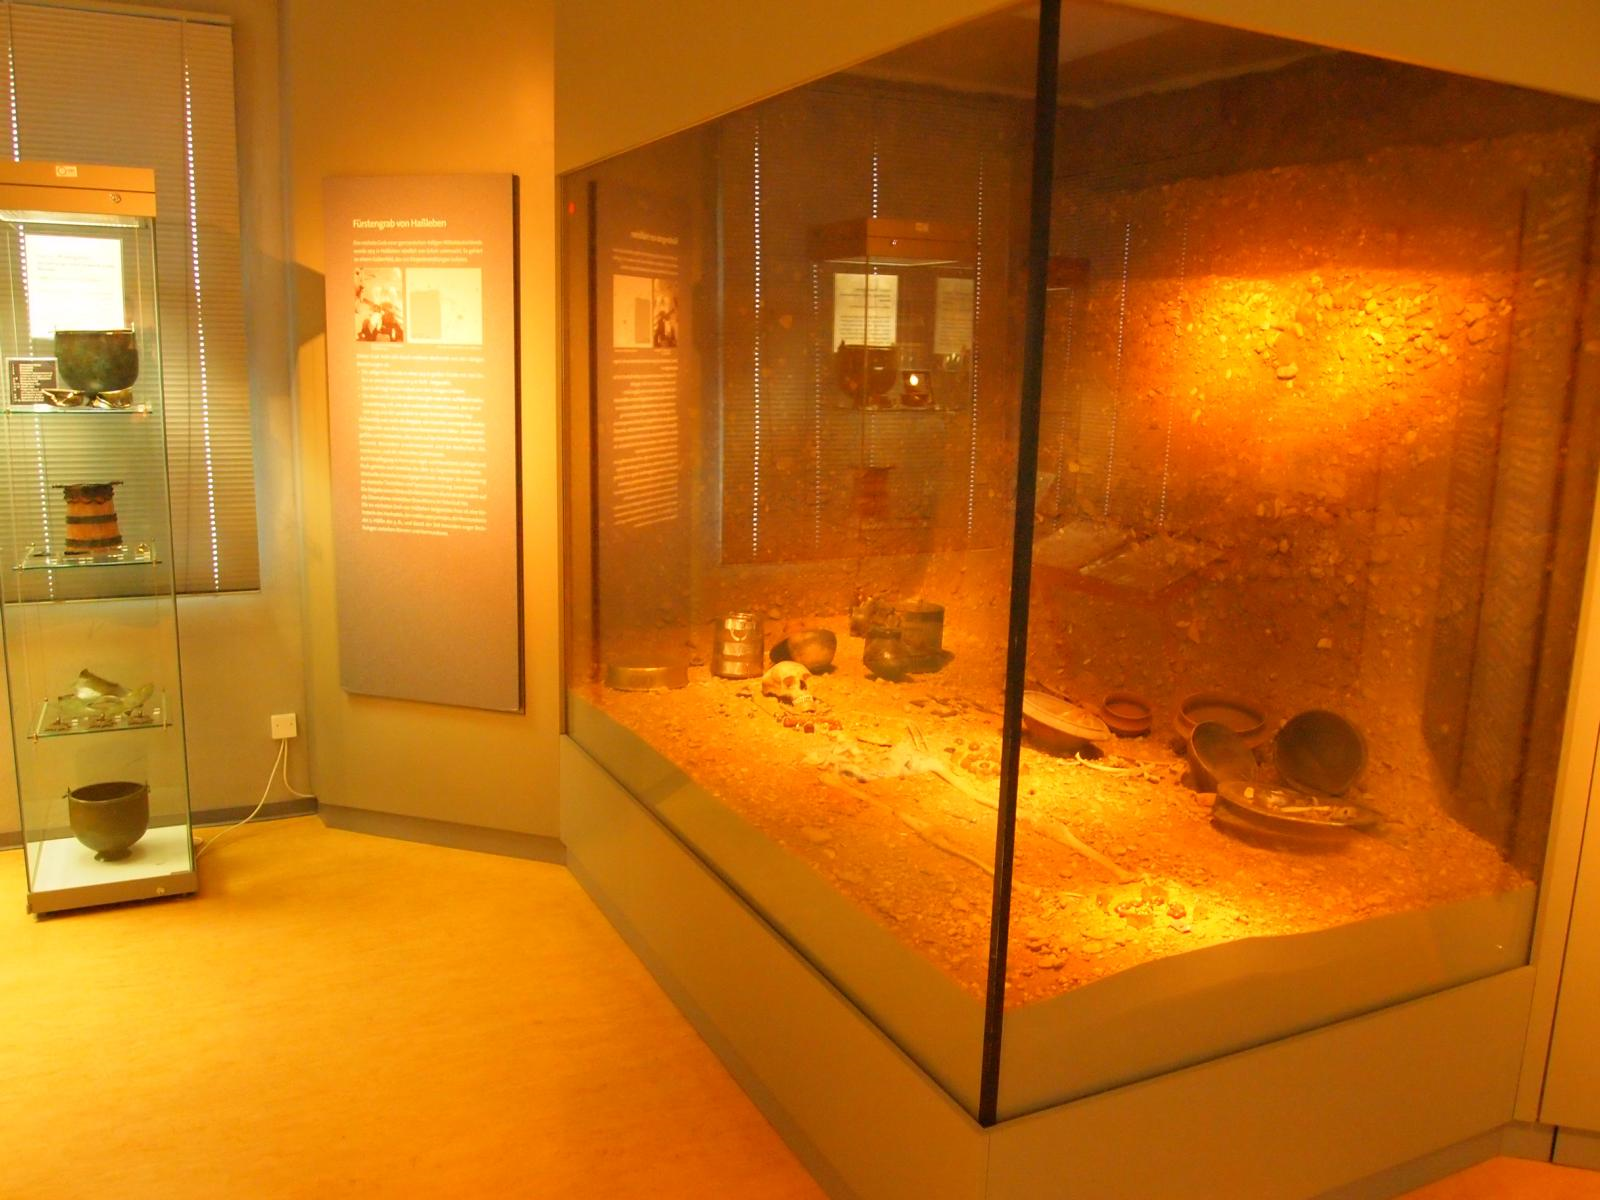
\includegraphics[scale = 0.7]{../pics/Original.eps}
	%\caption{Fürstengrab von Haßleben-showcase prior to installation.}
	%\label{fig:conception_grave}
%\end{figure}

According to the aforementioned review, the Fürstengrab von Haßleben was most promising and therefore chosen in the end. It contains many special relics from ordinary, Teutonic pottery to rare, Roman coins and jewelry. There are original artifacts and replicas on display inside the showcase, which I am collectively referring to as \textit{exhibits} throughout this work. Some of these exhibits are shown in Figure \ref{fig:conception_grave}a, b and c. The apparent eclecticism is, what makes the grave so special though. It is a sublime showcase for thriving trade and cultural exchange between Teutons and Romans as far east as Thuringia. Further, it proves how Teutons began adapting roman traditions, such as burials. In order to emphasize this insight, an interactive system was to be developed. Unfortunately, the showcase is located on the second floor. Thus, it does not get the attention it deserves. People are often tired after having visited the first floor. Hence, the museum's staff asked for an installation that would reactivate the visitors' attention.

%---------------------------------------------------------------------------- 

\section{System Preconditions}
\label{conception_system}

The system was to be developed and tested by me, and the museum-staff is responsible for its future maintenance. The full range of visitors' backgrounds cannot be foreseen. Some visitors might not have the proper technical experiences to operate contemporary interfaces. Consequently, it was crucial to design the system with that in mind. It had to be operable by absolute lay persons, who have no prior experience concerning information technologies. Hence, the interface had to be as intuitive and natural as possible. Four major points had to be considered.
\\
First, established and abstract input devices, such as keyboard and mouse, had to be replaced by something more natural. In order to be intuitive, the interaction was designed to capture and use the natural behavior of visitors. Outputs, on the other hand, had to be as discreet and as conservative as possible to not disturb or interfere with the exhibition. Thus, invasive technologies such as speakers and animatronics were excluded by the museum from the beginning. This consideration only left visual and haptic channels for output. The third point was, that daily operations at the museum were not to be compromised. So, it was not possible to develop the prototype inside the Haßleben-showcase itself and a full-size mockup had to be build somewhere else. Furthermore, the showcase and its precious exhibits had to be protected from any possible decay and nothing was to be rearranged. Thus, I measured the showcase and acquired a room in which a mockup could be placed for the prototype's implementation and testing\footnote{For a further description of the lab-setup see Chapter \ref{setup_development}}. Finally, the system's components, in- and output devices, had to be robust enough to cope with daily use. Moreover, they should also stay in their intended place. This meant that they had to be somehow attached to the showcase.

In summary, the requirements for the final system were narrowing down the possibilities right from the beginning. Hence, we came up with several ideas and followed up on all of them, until one promised to be the most feasible.

%\paragraph{Annotations}
%
%\begin{itemize}
	%\item User perspective
	%\begin{itemize}
		%\item Visitor
		%\item Curator / staff
	%\end{itemize}
	%\item System view
	%\\
	%\item Development of ideas according to the plan
	%\begin{itemize}
		%\item Method of elimination
		%\item Feasibility
		%\begin{itemize}
			%\item Effort
			%\item Cost
		%\end{itemize}
	%\end{itemize}
%\end{itemize}

%-----------------------------------------------------------------------------

%\paragraph{Annotations}
%
%\begin{itemize}
	%\item Possibilities of hard- and software
	%\item Capabilities of a single programmer (me)
%\end{itemize}

%-----------------------------------------------------------------------------

\section{Concept Development}
\label{conception_constraints}

Developing the system, we followed two initial approaches. They were supposed to lead us to an intuitive, easy to use interface, which would be very naturally operable. The first concept featured the development of tangibles. Interactive objects would be placed outside the showcase and visitors would be able to interact with them. Haptic feedback would enable visitors to experience the exhibits in an unusual way. By touching replicas of otherwise locked up exhibits a deeper involvement is highly likely. Meanwhile, the other concept was based on gestural interaction. With this concept, visitors are enabled to interact with the showcase by pointing. This approach was based on the natural behavior of visitors. Like the previous approach an uncommon experience should raise visitors' involvement and attention.

\paragraph{Tangibles} 

The early idea behind this work was to work with \ac{MS} Gadgeteer to develop a tangible interface for and with a museum. Thus, we first thought about how to include those Gadgeteer-modules. Therefore, I built the demo device shown in Figure \ref{?}, which was based on a \textit{FEZ Spider Starter Kit}~\cite{SpiderKitGHI}. In addition, it utilized an \ac{RFID}-reader~\cite{RFIDreaderGHI} and a potentiometer~\cite{PotentiometerGHI}. The RFID-transponders were attached to an old 2,5" \ac{HDD} and a wireless mouse. When the \ac{RFID}-tags were recognized, an image of the object was displayed on the screen. By turning the potentiometer's knob the angle of view changed accordingly. This gave an impression of the possibilities of the hardware. Unfortunately, we only had two \ac{RFID}-tags that had the size of a credit card. After some research though, I found some tags for the correct frequency band and in sizes from a grain of rice over credit cards to key chains~\cite{RFIDtransponder}. Hence, including \ac{RFID}-tags in tangibles was feasible. 
\\
The shape and size of the tangibles were still up for debate. Another point was, whether the hardware would be placed inside or outside the tangibles. This decision dictates the shape and size of the tangibles and therefore the interaction. If it would be placed inside, the tangibles would have to be big. They would have turned out at approximately the size of a box of milk. Such an \textit{active tangible} would be handy and a whole system could be concentrated in one device. On the other hand, they would be prone to damage and maybe even theft. Hence, the tangibles would have to be tough and in some way attached to the showcase. In addition, batteries would have to be either charged or changed. This would take a certain amount of maintenance.
\\
With the hardware outside the tangibles and hidden in a pedestal in front of the showcase, the tangibles could be smaller. Moreover, \textit{passive tangibles} grant more flexibility concerning the shape as well. As described earlier (see Chapter \ref{motivation_interfaces} in ~\cite{TangibleUI}), the tangibles could have different features depending on certain properties. In this case, several \ac{RFID}-tags could be placed in each tangible. Depending to their \textit{constrained} collocation on the \ac{RFID}-reader, different reactions of the system could be triggered. In contrast to Ullmer at al., 2005, though, this affordance would be hidden and thus less obvious. The tangibles would have to be attached to the pedestal as well, although they would be less expensive to replace.

Both approaches had their advantages and disadvantages and none of them was concrete enough to make a decision. Thus, we continued to specify the concepts depending on their strengths and weaknesses. We did this, by anticipating probable relations between the exhibits inside showcase and the behavior of visitors behind the glass. There are several things visitors tend to do, if they are interested in an exhibit. They would like to inspect it up close. First, this means they would like to touch an exhibit and feel it. Second, they want to see it in more detail and from different angles. Next and induced by restrictions, visitors talk about an exhibit or  request further information. This could be anything from its age to where and how it was found.
\\
An active tangible could provide nearly all of those qualities in one package. It could - like the demo device - be fitted with a display and an \ac{RFID}-reader. The corresponding \ac{RFID}-tags could then be placed close to the device in order to trigger a particular output. Those outputs could be saved either on the device itself or provided by a server. The question of how to trigger different reactions was to be answered next. The device could either be placed on a pedestal equipped with \ac{RFID}-tags or the tags had to be brought to the reader in any other way. As mentioned earlier, an active tangible would be sizable and it would have to be related to the showcase's topic as well. Hence, it would be reasonable to combine those two criteria and fabricate enlarged reproductions of exhibits from the showcase. In order to fit the whole hardware, an active tangible would have to have a simple shape. This unfortunately excluded several of the more interesting exhibits, such as coins, a golden ring and other jewelry. Some options remained though. There was a skull, pottery and the metal remains of two jewelry boxes.
\\
The passive tangibles did not appear to cause this much consideration. Any exhibit could have been \ac{3D} scanned\footnote{The scans could have been done in the labs of the chair of Computer Vision and Engineering at Bauhaus-Universität Weimar.}, turned into a digital model, appropriately altered to fit an \ac{RFID}-tag and then printed or milled out. The printed or milled reproduction could be used as a positive to produce casting molds, afterwards. Thus, replacing damaged or otherwise lost tangibles would be more cost-efficient. In addition, it could be done by the museum-staff themselves. One or more \ac{RFID}-readers could be placed in a pedestal in front of the showcase. Depending on the \ac{RFID}-reader and a tangible's tag, the system would display the corresponding output.
\\
During those considerations, a third possibility came up. A hybrid approach that combined both principles was possible as well. The reproduction of a jewelry box could be turned into an active tangible and passive tangibles could be put inside to trigger an output. The \ac{RFID}-reader would be placed underneath the box's floor and the display in the lid. In order to provide different types of content, we thought about also producing two different types boxes. A more or less \textit{authentic reconstruction} made of wood and metal fittings could provide authentic information about a passive tangible's cultural background. Meanwhile, the other box could be constructed of transparent material, which would allow the user to see the hardware. This \textit{futuristic reconstruction} could provide statistical content for the same passive tangible.

However, the main problem remained with all approaches. Some kind of pedestal would have to be built and placed outside the showcase to hold the active and/or passive tangibles. Although passive tangibles would have been more cost-efficient to replace than active ones, maintenance was rated too high. Furthermore, if the pedestal was not to obscure the showcase, it would have been too low\footnote{The height of the showcase floor is about 65cm. For more details see Chapter \ref{installation}.} to grant satisfactory access for any visitor.

%-----------------------------------------------------------------------------

\paragraph{Pointing}

%As a result of the earlier drawbacks, we tried to minimize the objects outside the showcase. Hence, the display should be put inside.

The alternate concept took a completely different approach. It was more related to \ac{VR} and the interaction in \ac{3D} environments, where users are pointing at an object to select it~\cite{VRObjectSelectionCnG}. The underlying idea was to develop an information system that would be based on pointing-based interaction. A user points at an exhibit inside the showcase, the system recognizes the gesture, calculates the intended target and displays the corresponding information.
\\
Since the display should not interfere with the exhibits or occlude them, we had to make decisions about the position, size and type of the display. In order to not occlude exhibits, the display should not be placed in front or above the exhibits. Directly behind the glass panel would also have been problematical. It should have been placed along the visitors' viewing direction as they already would be looking into the showcase. This way, it would still imply coherence through visual proximity. A monitor on the one hand, and a projector on the other were two possible technologies to choose from. Both came with their own challenges. While a projector would have been easier to conceal than a monitor, a monitor would produce less heat and noise. Because most of the visitors approach the showcase from the long side and tend to stay there for most of the time, the display should be visible from this direction. This meant placing the projection plane or display on the opposing wall. Another solution for a projector came up during this consideration. A \ac{PDLC} switchable film~\cite{PDLC} could have been placed on the glass panel. Whenever the system was activated, the film and projector could have been activated as well\footnote{A \ac{PDLC} switchable film can be switched between a transparent and an opaque state. In its opaque state, it can be very well be used as a projection surface~\cite{PDLC}.}. Unfortunately, this solution would have been too expensive and difficult to install. A projection in the other direction was also disregarded, because the cost and heat issues caused by a projector were considered to high. Heat produced by a projector causes issues regarding the artifacts' conservation and is a safety risk for the sealed showcase. Therefore, we decided to install an LED-screen. It should be placed inside the showcase close to the exhibits.

\textit{Object selection in \ac{VR}-environments}~\cite{VRObjectSelectionCnG} and the \textit{SMSlingshot}~\cite{SMSlingshot}, nearly always use a \textit{pointing device} of some sort. With such a device, a potential user could directly point at the original exhibits within the showcase and trigger the corresponding reaction of the system - displaying related information. As described in detail in Chapter \ref{evaluation_pre}, I observed interactions between visitors and the showcase as well as between each other. During the pre-study, it turned out that visitors often pointed at the particular exhibits they were talking about. The interface could be designed to emulate this natural interaction between visitors and incorporate of the natural behavior.
\\
The first intention was to rebuild the SMSlingshot with Gadgeteer-hardware. The tangible was equipped with a microcontroller, a small display, a keyboard, a green laser, a wireless transmitter and of course batteries. A PC was used to put all the information together and render the output. Therefore, it had a camera to track the point a user was aiming at and a corresponding transmitter to receive the fired messages~\cite{SMSlingshot}. All those modules could be provided by Gadgeteer except the laser. A laser could have been controlled with a \textit{Breakout module}~\cite{BreakoutGHI} and a relay. However, shooting a laser into the showcase was a delicate issue. Hence, this solution had to be revisited, because for safety reasons it was not feasible. There could have been injuries of visitors' eyes or some of the precious exhibits might have reacted to the laser's energy in a corrosive way. We did not want to take those risks, but we were very keen on the idea of pointing interaction. Thus, I looked for other tracking methods. We could have used a tracking system similar to the aforementioned ones used in \ac{VR}. Those systems are expensive to install and maintain, though. Moreover, a proper compatibility with Gadgeteer was doubtful. So, I started looking for alternatives to Gadgeteer, too. Two established systems immediately came to mind. First, the \textit{Nintento Wii}, which uses a wireless device with pointing capabilities and additional inputs. Second, the \textit{\ac{MS} Kinect}, which is able to recognize free-hand gestures and might not require any device. Both are comparably inexpensive to acquire, have experienced support and communities and use less dangerous \ac{IR} light.
\\
The decision between the two was made according to the same criteria as mentioned above. Pointing with no device should be a more intuitive way to interact with the exhibition and other visitors than any handheld device. Furthermore, the restraint to use the system should be reduced. No tangible or pedestal would have to be created and attached to the showcase, which decreased cost for maintenance. Hence, the \ac{MS} Kinect was chosen.
\\
There is a Kinect for \ac{MS} Windows along with a special \ac{SDK} for \ac{MS} Visual Studio. As it turned out, the hardware inside the \ac{MS} Kinect was developed by \textit{PrimeSense} and is also used by the \textit{ASUS Xtion PRO}. This \ac{3D}-sensor is less expensive and smaller, which allows to be less intrusive inside the showcase. Besides, we already had some of them at the faculty, which meant that I could start developing right away. Another change was the decision for an open source \ac{SDK} called \textit{OpenNI}\footnote{OpenNI was co-founded by PrimeSense, a hardware developer that produces \ac{3D} sensing hardware. In November 2013 PrimeSense was bought by Apple, whereupon OpenNI was shut down.}, which in combination with its add-on \textit{NiTE} enabled me to use \textit{skeleton tracking}. This was critical for my approach, because I needed to have a \ac{3D} vector in order to be able to calculate where a user was pointing. Skeleton tracking would deliver the joints of a tracked person. Hence, I was able to retrieve the directions a limb is oriented in. If this vector was extended, I was able to calculate its possible intersection with an exhibit. More about used software and the exact calculations can be found in the next chapter.

The last topic that needed addressing was \textit{feedback}. Since there would be no haptic or acoustic feedback, and no \textit{glowing dot} produced by a laser either, future users would need another visual feedback in order to be able to see where they were pointing and determine how to correct that. Once more, Gadgeteer could have provided a solution. Our first idea was to replace the laser's dot by a spotlight. The system would calculate the position a user was pointing at and transmit it to a Gadgeteer-system. It would then move a special highlight to this position within the showcase. Only two actuators would be sufficient. The maintenance of this kind of installation could become very complicated though, because the system would have to be installed on the ceiling of the showcase. Actuators need to be calibrated regularly and mechanical gearing will wear out. Hence, this realization concept was dismissed. Nevertheless, the principle should remain the same. Thus, the aforementioned position would now be shown on an overview of the showcase on the display.

%\paragraph{Annotations}
%
%\begin{itemize}
	%\item Technical
	%\item From the museums perspective
	%\begin{itemize}
		%\item Size
		%\item Cost
		%\item Inclusion
	%\end{itemize}
	%\item Limitations of hard- and software
	%\item Capabilities of a single programmer (me)
%\end{itemize}

%-----------------------------------------------------------------------------

\section{Final Concept}
\label{conception_final}

%\textbf{Soll ich hier nochmal das Gesamtkonzept zusammenfassen oder ist es besser, das Organisatorische noch etwas mehr zu vertiefen und dafür das fertige System im Implementation-Kapitel genau zu erklären? -- Dann muss ich hier nochmal die Überschrift ändern.}

The final system consists of a \textit{depth sensor}, a \textit{PC} and a \textit{display}. All of the hardware is placed inside the showcase. In addition, an active tangible to remotely activate and deactivate the system should be developed as well. It was only intended to be a feasibility study, which determines if and how active Gadgeteer-tangibles might be incorporated into the system, later. Suitable components were recommended by me and provided by the museum after to mutual agreement.

The system requires two pieces of software. The first software is of an administrative nature and allows the museum staff to define and maintain the whole exhibition. The second software is presenting the exhibition to the visitors. Previously defined exhibits are selectable.
\\
The exhibition can be defined by museum-staff themselves. Therefore, an exhibition plane has to be defined and validated first. After that all the exhibits' positions on the plane can be defined and validated. Those positions can be defined in the same way users later interact with the system, by pointing. To exclude a certain inaccuracy when defining a position, it would have to be defined from different angles and validated afterwards. The whole process will be described in Chapter \ref{installation} and the technical execution in Chapter \ref{installation_tech}. Furthermore, the corresponding contents such as explanatory texts and detailed images are provided by the staff. Contents and positions can be changed, removed from or reloaded into the exhibition.
\\
When one or more visitors enter the area in front of the showcase the system recognizes them and reacts in an inviting fashion. A defined interaction space enables the user to interact with the system by pointing at an exhibit. No devices outside the showcase are needed. 

\paragraph{Functional Specification Document (\ac{FSD})} The final concept all parties agreed on was written down by me in an \ac{FSD} and responsibilities were covered by a contract. The document states, which features of the final system must, should and must not be implemented and working.
\\
The necessary features or \textit{must-criteria} where that the the system would have to have separate modes for administration and presentation of an exhibition. The visual feedback of the interaction would be provided by the display. Visitors would be automatically recognized by the system, but only one user at a time would be able interact with it. The whole system would be maintainable by the museum's staff and will start and shut down automatically.
\\
Preferable features \textit{should} be realized, but would not be mandatory. Thus, there should be a system's manual. For guided tours, it should be further possible to switch the system into a 'blind' mode, where it does not react to people. Extensive exhibits should have a slide show. The system should be operable with either the left or right hand. In addition, statistics about the system's use should be logged for later analysis.
\\
There were also criteria that were not requested, and therefore \textit{must not} be implemented. Any free-hand gestures other than pointing must not be recognized by the system. Further, the lighting inside the showcase must not be controlled or influenced by the installation. Feedback has to be only visual and not auditive or haptic. Hence, speakers or tangibles must not come to use. 
\\
Furthermore, the \ac{FSD} describes system requirements concerning hard- and firmwares, data formats and other organizational parameters. 

In addition to the \ac{FSD}, a contract was drawn up by the university's layer's office. It sorted responsibilities and was later signed by the museum's director, my professor and me. Both documents can be found in the appendix.

%\paragraph{Annotations}
%
%\begin{itemize}
	%\item 'Pflichtenheft'-criteria
	%\begin{itemize}
		%\item Must
		%\begin{itemize}
			%\item 
		%\end{itemize}
		%\item Should
		%\begin{itemize}
			%\item 
		%\end{itemize}
		%\item Could
		%\begin{itemize}
			%\item 
		%\end{itemize}
		%\item See appendix
	%\end{itemize}
	%\item Contract 
		%\begin{itemize}
			%\item MUFT, BUW and me
			%\item Avoid misconceptions
			%\item Commitments / Obligations
			%\item Responsibilities
			%\item Boundaries
			%\item Legal stuff
			%\item See appendix
		%\end{itemize}
%\end{itemize}
